% Intended LaTeX compiler: pdflatex

        \documentclass{beamer}
\usetheme{metropolis}
\institute{Mentorsprogram i matematik}

    \usepackage[T1]{fontenc}     
    \usepackage[utf8]{inputenc} 
    \usepackage[swedish, english]{babel}
    \usepackage{amsfonts}
    \usepackage{amsmath}
    \usepackage{amssymb}
    \usepackage{hyperref}
    \newcommand\NN{\ensuremath{\mathbb{N}}}
    \newcommand\RR{\ensuremath{\mathbb{R}}}
    \newcommand\ZZ{\ensuremath{\mathbb{Z}}}
    \renewcommand\O{\ensuremath{\\emptyset}}
    \newcommand\QQ{\ensuremath{\mathbb{Q}}}
    \newcommand\CC{\ensuremath{\mathbb{C}}}
    \usepackage{import}
    \usepackage{xifthen}
    \usepackage{pdfpages}
    \usepackage{transparent}

    \newcommand{\incfig}[1]{%
        \def\svgwidth{\columnwidth}
        \import{./img/}{#1.pdf_tex}
    }
\usepackage[utf8]{inputenc} 

\usepackage[T1]{fontenc} 

\usepackage{amsmath} 

\usepackage{amssymb} 

\usepackage{enumerate} 

\usepackage{prftree} 

\usepackage{mathpartir} 

\usepackage{mathtools} 

\usepackage{stmaryrd} 

\usepackage{color} 

\definecolor{darkgreen}{rgb}{0,0.45,0} 

%\usepackage[colorlinks,urlcolor=darkgreen,linkcolor=darkgreen]{hyperref} 

\makeatletter 

\newlength{\tempwidth@narrowinferruleconcl} 

\newcommand{\narrowinferrule}[4][0pt]{% 

  % Optional argument #1: optional extra padding 

  % Compulsory arguments #2–#4: arguments of \inferrule* (but optional arg of that is compulsory here) 

  \settowidth{\tempwidth@narrowinferruleconcl}{$#4$}% width of conclusion 

  \mathmakebox[\tempwidth@narrowinferruleconcl+#1][c]% 

    {\inferrule*[right=\protect{\rlap{#2}}]{#3}{#4} \hspace*{-1.4ex}}%  

  } 

 

\newcommand{\negphantom}[1]{\settowidth{\dimen0}{#1}\hspace*{-\dimen0}} 

\makeatother 

 

\newcommand{\todo}[1]{\textcolor{red}{#1}} 

 

% styled letters 

\newcommand{\A}{\mathcal{A}} 

\newcommand{\D}{\mathcal{D}} 

\newcommand{\N}{\mathbb{N}} 

\newcommand{\cN}{\mathcal{N}} 

\newcommand{\R}{\mathbb{R}} 

\newcommand{\cR}{\mathcal{R}} 

\newcommand{\Z}{\mathbb{Z}} 

\newcommand{\V}{\mathcal{V}} 

\newcommand{\Q}{\mathbb{Q}} 

\newcommand{\cQ}{\mathcal{Q}} 

% binary relations 

\newcommand{\proves}[1][]{\mathrel{\vdash_{#1}}} 

\newcommand{\notproves}[1][]{\mathrel{\nvdash_{#1}}} 

\newcommand{\entails}[1][]{\mathrel{\vDash_{#1}}} 

\newcommand{\notentails}[1][]{\mathrel{\nvDash_{#1}}} 

\newcommand{\believes}[1][]{\mathrel{\vDash_{#1}}} 

\newcommand{\notbelieves}[1][]{\mathrel{\nvDash_{#1}}} 

\newcommand{\logequiv}{\approx} 

 

% syntax of logic 

\newcommand{\limp}{\rightarrow} 

\newcommand{\liff}{\leftrightarrow} 

\newcommand{\ltrue}{\top} 

\newcommand{\lfalse}{\bot} 

\renewcommand{\land}{\wedge} 

 

% miscellaneous 

 

\renewcommand{\Form}{\mathrm{Form}} 

\newcommand{\Term}{\mathrm{Term}} 

 

\newcommand{\signature}[1]{\langle\, #1\, \rangle} 

\newcommand{\strux}[1]{\langle\, #1\, \rangle} 

\newcommand{\nextpart}{\,\mathpunct{;}\,} 

\newcommand{\interp}[2][]{\llbracket\; #2\; \rrbracket^{#1}}
\author{Vetenskapens Hus}
\date{December 15, 2021}
\title{Introduktion till analys}
\hypersetup{
 pdfauthor={Vetenskapens Hus},
 pdftitle={Introduktion till analys},
 pdfkeywords={},
 pdfsubject={},
 pdfcreator={Emacs 28.1 (Org mode 9.5.2)}, 
 pdflang={English}}
\begin{document}

\maketitle



\section*{Funktioner}
\label{sec:orga35961a}
\begin{frame}{En funktion är en regel}
\begin{itemize}
\item En funktion är en regel som för varje tal ger ut ett nytt tal.
\item Vi betecknar ofta funktioner med bokstäver
\end{itemize}
\textbf{Exempel:}
Om vi definerar \(f\) som:
\begin{align*}
f(x) = x^2 + x
,
\end{align*}
då betyder det att t.ex.
\begin{align*}
f(3) = 3 ^2 + 3 = 9 + 3 = 12
.
\end{align*}

\textbf{Fråga:}
Vad är \(f(2)\) likamed?
\end{frame}

\begin{frame}{Vi kan symbolisera funktioner med grafer}
Om vi ritar ut alla punkter där \(f(x)=y\) så får vi
en användbar graf. I detta exempel så är \(f(x) = x^2\) igen.
\begin{center}
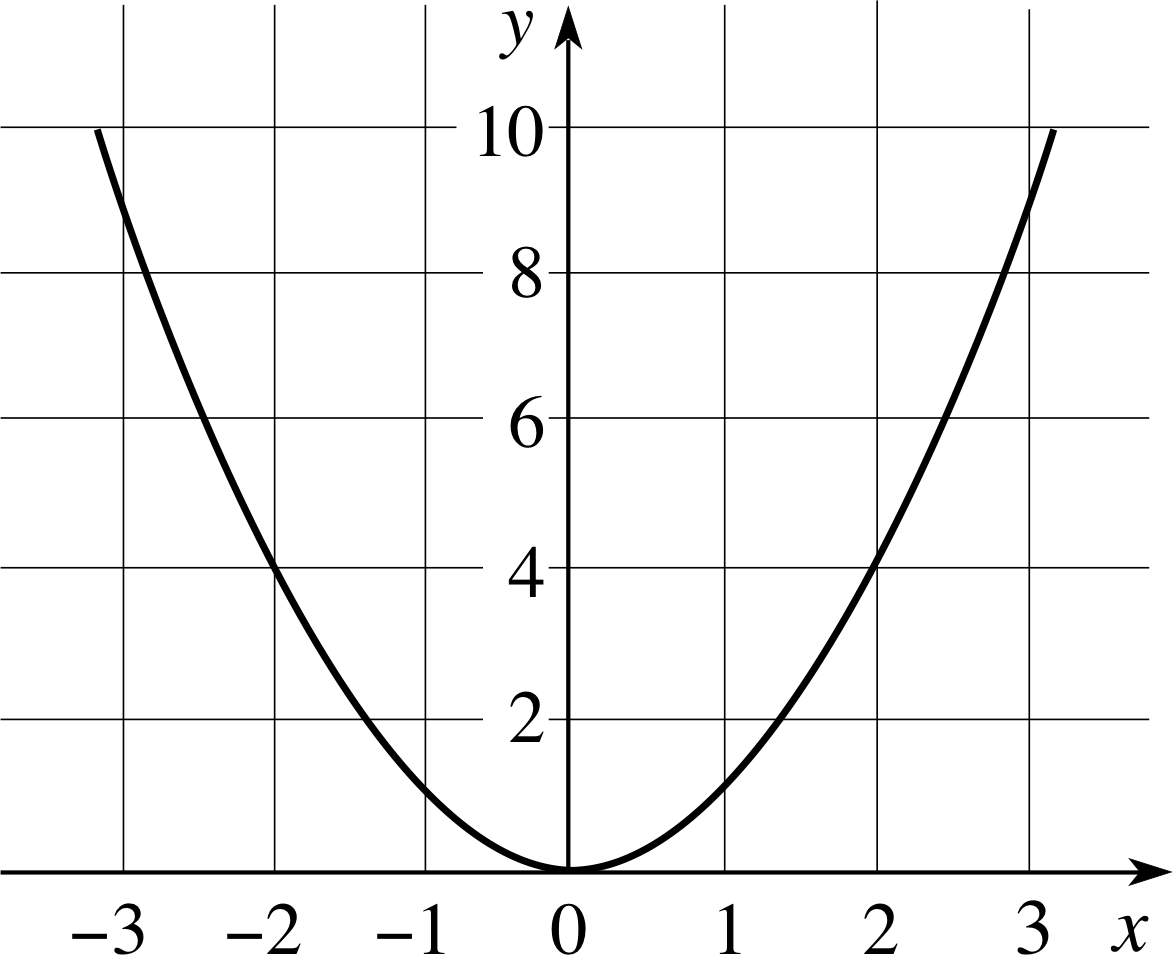
\includegraphics[angle=0,width=5cm]{./img/squared.png}
\end{center}
\end{frame}

\subsection*{Frågor: funktioner}
\label{sec:orge3b3e25}
\begin{frame}{Frågor: funktioner}
\textbf{Fråga 1:} Om \(a(x) = x - 3\) och \(b(x) = 4\) vad är då 
\(a(2) + b(3)\) likamed?
\newline
\textbf{Fråga 2:} Om \(a(x) = x^2+1\) och \(b(x) = 0\) vad är då 
\(a(1) + b(-1)\) likamed?
\newline
\textbf{Fråga 3:} Om \(a(x) = 5 - x\) och \(b(x) = -1\) vad är då 
\(a(3) + b(2)\) likamed?
\end{frame}




\section*{Derivata}
\label{sec:orgafbd31c}
\begin{frame}{Derivata är lutning}
Vi säger att lutning på en linje är hur mycket du ändras om du
går ett steg åt höger.
\begin{center}
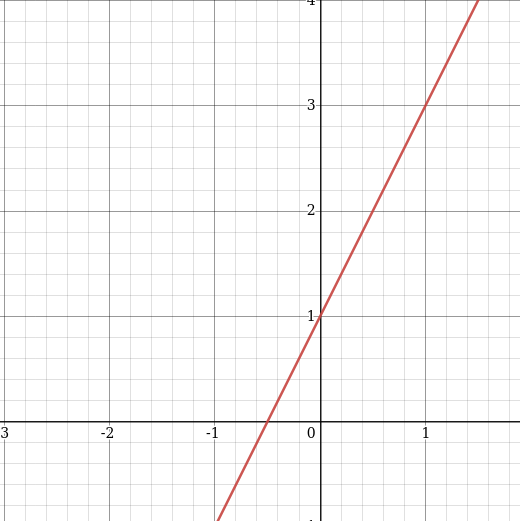
\includegraphics[angle=0,width=5cm]{./img/2x.png}
\end{center}
\end{frame}


\begin{frame}{Varför bryr man sig om lutningen?}
Lutningen kan tolkas som hastigheten om funktionen beskriver hur långt man har
åkt med t.ex. ett tåg.
\end{frame}


\section*{Integraler}
\label{sec:orgd645837}
\begin{frame}{Integralen är arean}
Om vi undrar vad arean mellan funktionen mellan två punkter
på \(x\) axeln så kallar vi det att vi tar integralen mellan de två punkterna.
\newline
\textbf{Exempel:}
Om vi har funktionen \(f(x) = 2\) (röd i grafen), så är
\begin{align*}
\int_{ 1 }^{ 3} f(x) dx = 4
.
\end{align*}

\begin{center}
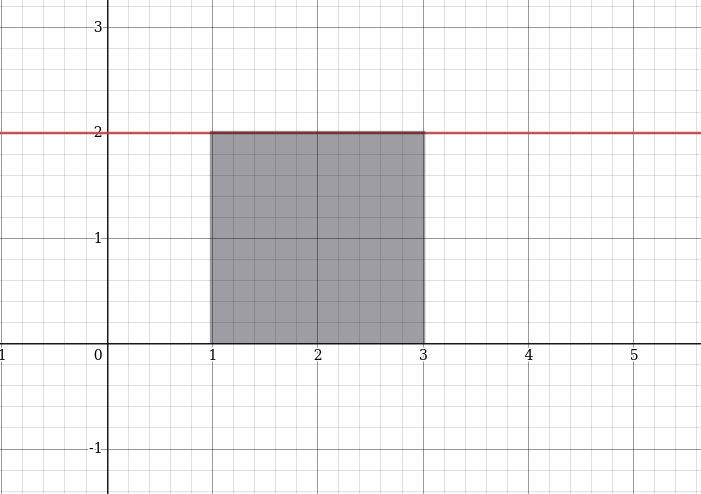
\includegraphics[angle=0,width=5cm]{./img/integral.png}
\end{center}
\end{frame}

\begin{frame}{Varför bryr man sig om arean?}
Om vi har att funktionen beskriver hur snabbt man åker vid en viss tidpunkt,
så säger integralen hur långt man hade åkt i intervallet man tar integralen.
\end{frame}


\section*{Analys}
\label{sec:org8fc3346}
\begin{frame}{Vad är analys (på engelska: Calculus)}
Analys (i matematik) är ett ämne i matematik där man löser problem
genom att använda \emph{oändligt små värden}.
\end{frame}

\begin{frame}{Exempel: derivata}
I de förra uppgifterna så hade våra funktioner samma lutning över
hela grafen. Men tänk om vi har en mer komplicerad funktion
som t.ex. \(f(x) = x^2\), hur gör vi då?
\begin{center}
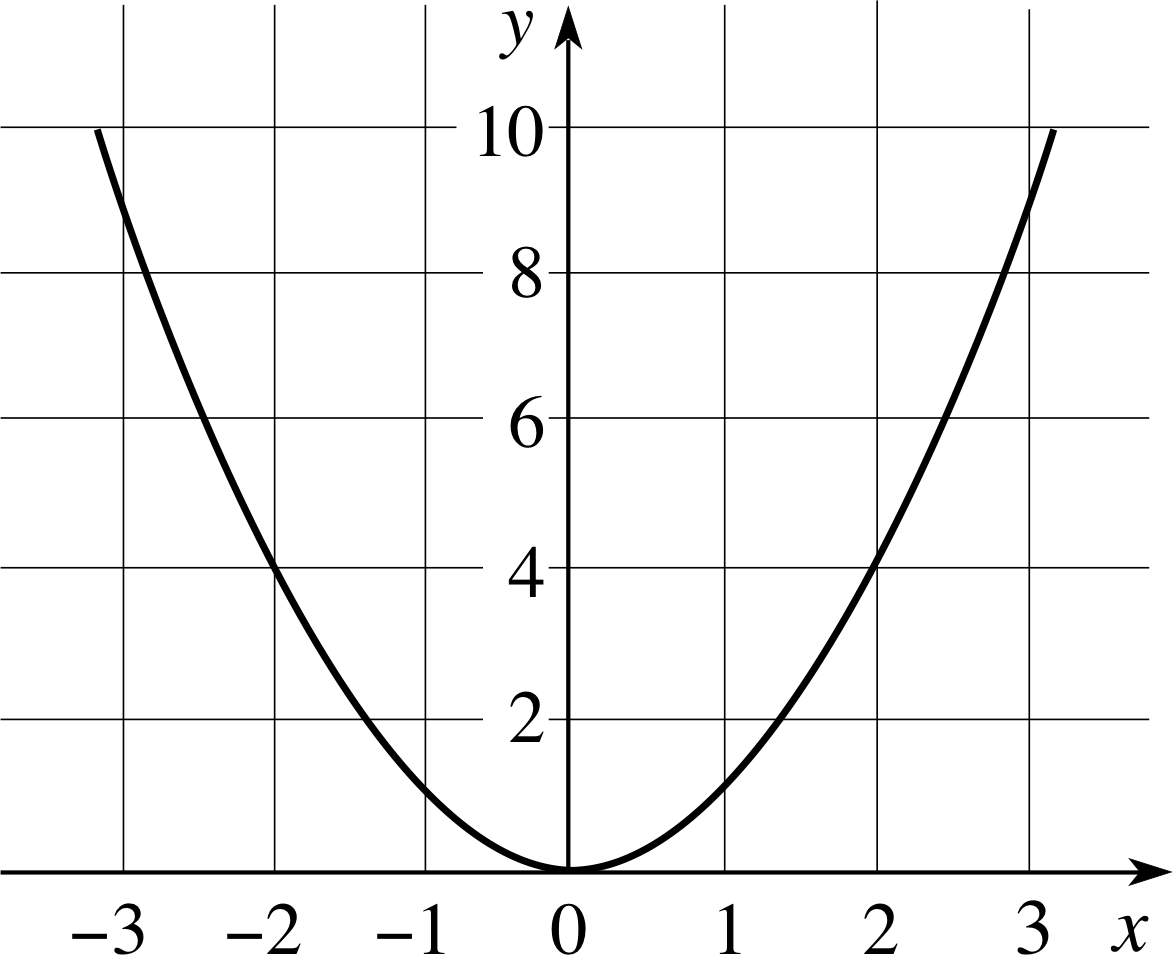
\includegraphics[angle=0,width=5cm]{./img/squared.png}
\end{center}
\end{frame}

\begin{frame}{Exempel: derivata}
\textbf{Lösning:} Vi kan få derivatan vid en specifik punkt genom att
zooma in oändligt mycket. \href{https://desmos.com/calculator}{Desmos}
\end{frame}

\begin{frame}{Exempel: integral}
Samma sak med integralen, om vi har t.ex. \(f(x) = x^2\) så är
det inte lika enkelt att räkna ut arean mellan två punkter.
T.ex. vad är arean mellan 0 och 2 här?
\begin{center}
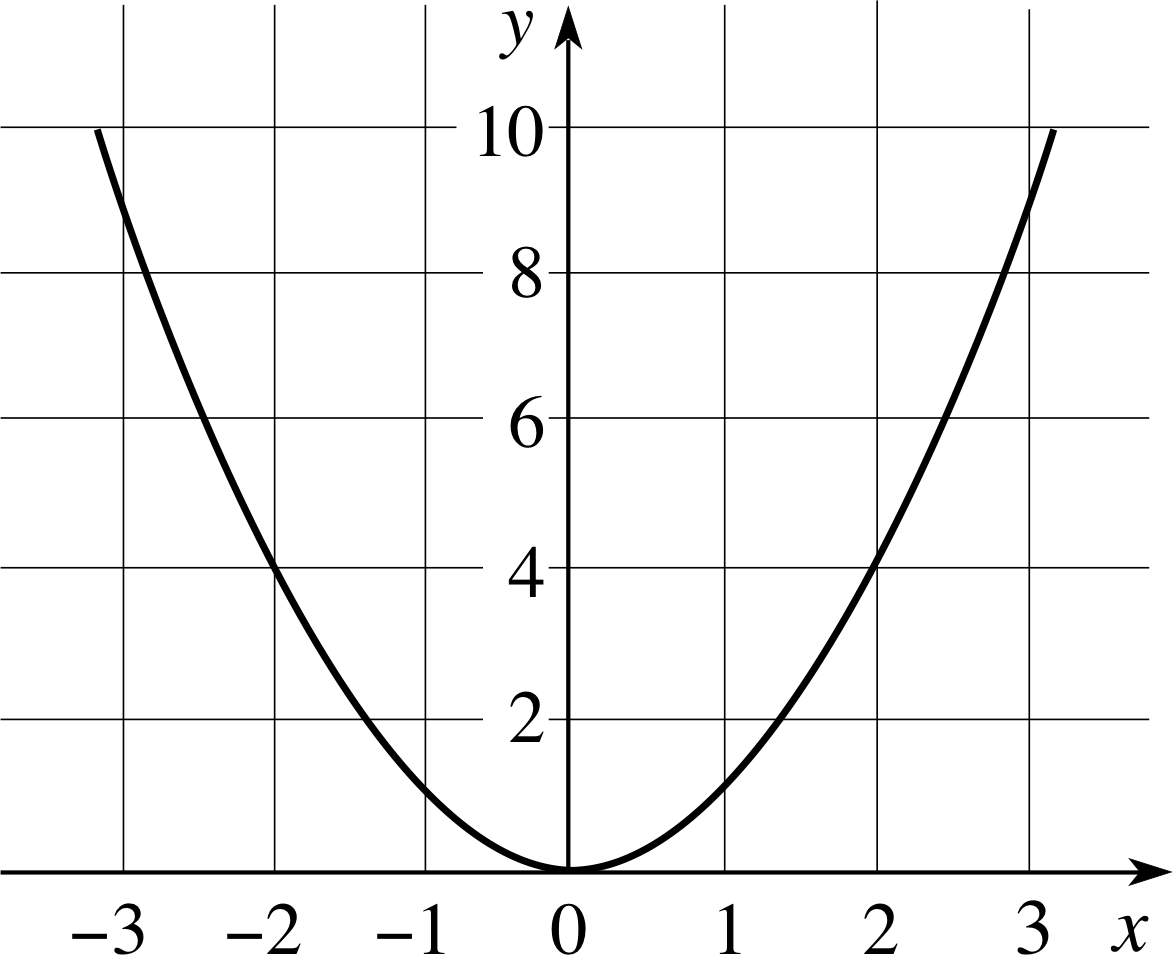
\includegraphics[angle=0,width=5cm]{./img/squared.png}
\end{center}
\end{frame}

\subsection*{Exempel integral}
\label{sec:org2feb6bc}
\begin{frame}{Exempel integral}
\textbf{Lösning:} Vi kan approximera arean med rektanglar.

\begin{center}
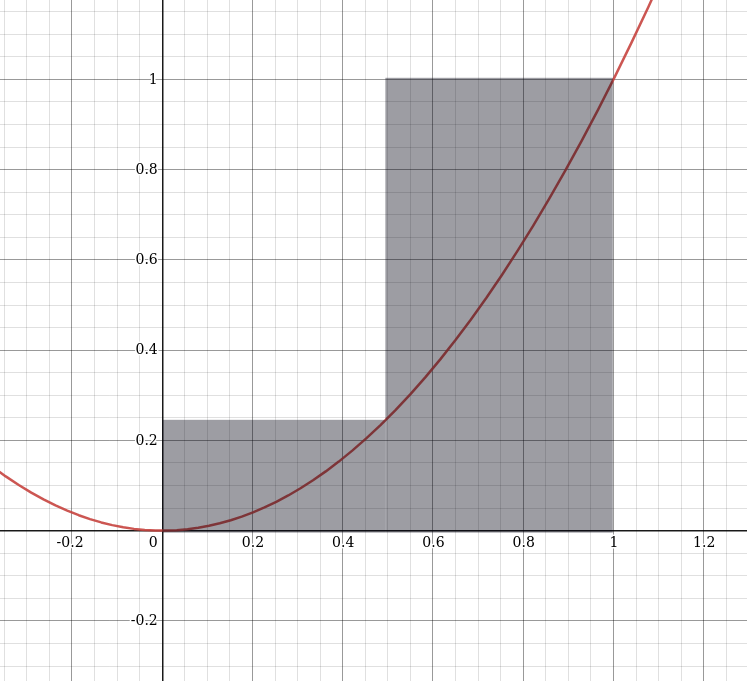
\includegraphics[angle=0,width=5cm]{./img/int2.png}
\end{center}

\end{frame}



\subsection*{Exempel integral}
\label{sec:org9a33b1c}
\begin{frame}{Exempel integral}
\textbf{Lösning:} Vi kan approximera arean med rektanglar.
\begin{center}
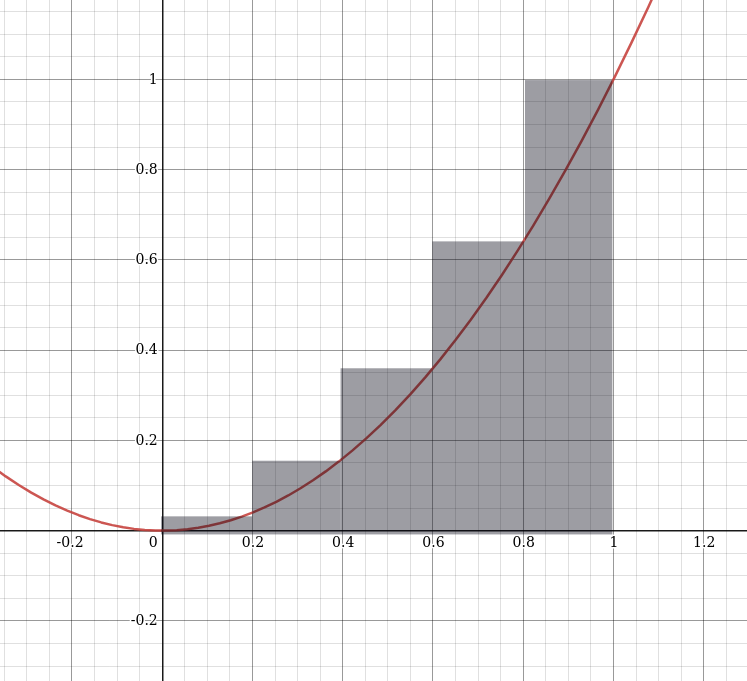
\includegraphics[angle=0,width=5cm]{./img/int5.png}
\end{center}

\end{frame}





\section*{Oändligheten}
\label{sec:orgc171ccb}
\begin{frame}{Det största talet?}
\begin{itemize}
\item Vad är ett tal?
\item Vi vill kunna avända operationer på tal (+-*/)
\item Injektiv under dessa operationer
\item Är oändligheten ett tal?
\end{itemize}
\end{frame}

\begin{frame}{Hur räknar man med oändligheten om vi låtsades att det var ett tal?}
Vad blir:
\begin{itemize}
\item \(\infty + 1\)?
\item \(\frac{2}{\infty}\) ?
\item \(\frac{\infty}{\infty }\)?
\end{itemize}
\end{frame}


\begin{frame}{Talföljder}
\begin{itemize}
\item Talföljder är bara funktioner där man kollar på när man sätter in
\end{itemize}
1,2,3,4\ldots{} (heltal)
\begin{itemize}
\item T.ex. talföljden \(1,4,9,16 \dots\) är ju bara funktionen \(f(x) = x^2\) och sedan
så räknar vi ut \(f(1), f(2), f(3), f(4) \dots\)
\end{itemize}
\end{frame}


\begin{frame}{Vad är \( \frac{\infty}{\infty } \) likamed?}
Så här har vi tre talföljder, och ni ska räkna ut de första tre talen, sen
det tioende talet och sen det 100:e talet. Ni får använda miniräknare.

\textbf{Talföljd 1:} \begin{align*}
f (x) = \frac{x - 3}{x^2}
.
\end{align*}
\textbf{Talföljd 2:} \begin{align*}
f(x) = \frac{x-3}{x}
.
\end{align*}
\textbf{Talföljd 3:} \begin{align*}
f(x) = \frac{x^2 - 3}{x}
.
\end{align*}

Vad tror ni \(\frac{\infty}{\infty }\) är likamed?
\end{frame}

\begin{frame}{Oändligheten är en riktning på tallinjen}
Så \(+\infty\) är som "öster" och \(-\infty\) är som "väster".
\end{frame}


\section*{Division med noll}
\label{sec:org6ddf76d}
\begin{frame}{Vad är division?}
Vi säger att \(\frac{12}{4} = 3\) eftersom vi måste subtrahera fyra från 12 tre gånger
innan vi får noll.
\begin{align*}
&  12 - 4 = 8 \\
&  8 - 4 = 4 \\
&  4 - 4 = 0
.
\end{align*}

Hur många gånger måste vi subtrahera noll från \(12\) innan vi får noll?
\begin{align*}
&  12 - 0 = 12 \\
&  12 - 0 = 12 \\
&  12 - 0 = 12 \\
 &  \vdots 
\end{align*}
\end{frame}

\begin{frame}{Så om man delar på noll får man oändligheten?}
Låt oss räkna ut några talföljder igen för att få perspektiv. Fast den här
gången ska ni räkna ut för när \(x=1, x=0.1\) och \(x= 0.001\). Ni får
ännu igen använda miniräknare.

\textbf{Talföljd 1:} \begin{align*}
f (x) = \frac{x}{x}
.
\end{align*}
\textbf{Talföljd 2:} \begin{align*}
f(x) = \frac{x^2}{x}
.
\end{align*}
\textbf{Talföljd 3:} \begin{align*}
f(x) = \frac{x}{x^2}
.
\end{align*}

Vad tror ni \(\frac{0}{0}\) är likamed?
\end{frame}


\section*{Gränsvärden}
\label{sec:orga107ff2}

\begin{frame}{}
Så när vi räknar ut saker som \(\frac{10}{2}\) så kan vi med stor
säkerhet säga att det är likamed \(5\). Men vi kan inte
göra det med saker som innehåller oändligheten eller
division med noll som \(\frac{\infty}{\infty }\) eller \(\frac{0}{0}\).


Men detta är ju ett stort problem, för när vi ville räkna ut
derivata och integraler så använda vi termer som "oändligheten"
och "oändligt nära noll".
\end{frame}

\subsection*{Så vad är problemet med \(\frac{0}{0}\) och \(\frac{\infty}{\infty}\)?}
\label{sec:orge1ed2aa}
\begin{frame}{Så vad är problemet med \( \frac{0}{0} \) och \( \frac{\infty}{\infty} \)?}
Problemet är ju att vi fick ju olika svar beroende hur snabbt
varje del gick till \(0\) eller oändligheten.
Låt oss kolla tillbaka till talföljderna där \(x\) gick mot noll.
\(\frac{x^2}{x}\) gick mot noll för att täljaren gick mycket
snabbare åt noll än nämnaren. Och 
\(\frac{x}{x}\) gick mot 1 för att täljaren och nämnaren båda
gick till noll lika snabbt.
\end{frame}

\begin{frame}{Gränsvärde}
Så även om \(\frac{x^2}{x}\) och \(\frac{x}{x}\) blir \(\frac{0}{0}\) när \(x=0\) så blir de olika när
de går mot noll. Vi skriver detta som följande:
\begin{align*}
\lim_{ x \to 0 } \frac{x^2}{x} = 0
\end{align*}
och
\begin{align*}
\lim_{ x \to 0 } \frac{x}{x} = 1
.
\end{align*}

Så \(\lim_{ x \to 0 }\) betyder "när \(x\) går mot noll". På samma sätt så kan
vi skriva \(\lim_{ x \to +\infty }\) för att säga "när \(x\) går mot oändligheten".
\end{frame}

\begin{frame}{Några gränsvärdesregler}
En av de viktigaste regelerna med gränsvärden är att om vi kan
bara helt enkelt sätta in värdet utan att få \emph{problem} så
får vi göra det.
\newline
\textbf{Exempel:}
\begin{align*}
 &  \lim_{ x \to 0 } 2x + 3 = 2\cdot 0 + 3 = 3. \\
 &  \lim_{ x \to 0 } \frac{x+12}{x+6} = \frac{0+12}{0+6} = 2. \\
 &  \lim_{ x \to 0 } x = 0.
\end{align*}
\end{frame}

\begin{frame}{Vad räknas som "problem"?}
Det som räknas som problem är när man stoppar in och får någon
av följande "farliga" uttryck:
\begin{align*}
\frac{0}{0}, \frac{\infty}{\infty}, \infty -\infty , 0 \times \infty , 0 ^{0}, \infty ^{0}, 1 ^{\infty}
.
\end{align*}
\end{frame}

\subsection*{Huvudstrategin i uträkning av gränsvärden}
\label{sec:org79f0086}
\begin{frame}{Huvudstrategin i uträkning av gränsvärden}
Tyvärr så är "farliga" uttryck ganska vanliga. Vår strategi för att lösa detta är
att skriva om uttrycket med algebra tills vi får ett uttryck som inte innehåller
några "farliga" uttryck.
\newline
\textbf{Exempel:}
Vi kan inte räkna ut
\begin{align*}
\lim_{ x \to 0 } \frac{6x}{3x} + x
\end{align*}
direkt eftersom då får vi \(\frac{6\cdot 0}{3\cdot 0} + 0 = \frac{0}{0} + 0\), som innehåller
ett av de här "farliga" uttrycken. Men vi kan förkorta \(x\) och få
uttrycket \(\frac{6}{3} + x\).
Och vi får inget problem om vi sätter in noll direkt här
då vi får \(\frac{6}{3} + 0\). Så därför så kan vi dra slutsatsen att det är likamed
\begin{align*}
\lim_{ x \to 0 } \frac{6}{3} + x = \frac{6}{3} + 0 = 2
.
\end{align*}
\end{frame}


\section*{Kort om formell defintion av derivata och integral}
\label{sec:org830abc5}
\begin{frame}{En varning om att man inte behöver förstå direkt}
Dessa formella definitioner kommer inte se väldigt intuitiva ut, men
det är lungt. Poängen med att visa dessa definitioner är att
vi har ett precist sätt att räkna ut dessa saker som verkade tidigare
inte så precisa och mer filosofiska.
\end{frame}

\begin{frame}{Derivatans definition}
Om vi har en funktion \(f(x)\) så kallar vi derivatan \(\frac{df}{dx}\) och vi
definerar den som följande:
\begin{align*}
\frac{df}{dx} = \lim_{ h \to 0 } \frac{f(x+h)-f(x)}{h}
.
\end{align*}
\end{frame}

\begin{frame}{Integralens definition}
Låt \(\Delta x = \frac{b-a}{n}\) och \(x_i = a + \Delta x \cdot i\), då definerar vi integralen som
\begin{align*}
\int_{ a }^{ b} f(x) dx = \lim_{ n \to +\infty } \sum_{ i = 1 }^{ n } f(x_i) \Delta x
.
\end{align*}
\end{frame}


\begin{frame}{Vidare läsning/videor att se}
\href{https://www.youtube.com/watch?v=WUvTyaaNkzM\&list=PLZHQObOWTQDMsr9K-rj53DwVRMYO3t5Yr}{Essence of Calculus (Youtube serie av 3blue1brown, han gör också många andra bra videor)}

\href{https://www.mathsisfun.com/calculus/introduction.html}{mathisfun introduction to calculus (hemsida)}

\href{https://www.adlibris.com/se/bok/analys-i-en-variabel-9789144067650?msclkid=fdec5fb7484513345f2c3e741ec46196\&utm\_source=bing\&utm\_medium=cpc\&utm\_campaign=BOK\%20-\%20Search\%20-\%20Generic\%20-\%20Student\%20Titlar\&utm\_term=Analys\%20i\%20en\%20variabel\&utm\_content=Student\%20Titlar}{Analys i en varibel av Persson och Böiers (Avancerad bok för Universitetet)}
\end{frame}
\end{document}
